\PassOptionsToClass{tikz}{standalone}
\documentclass{ppedt-docfig}
\begin{document}
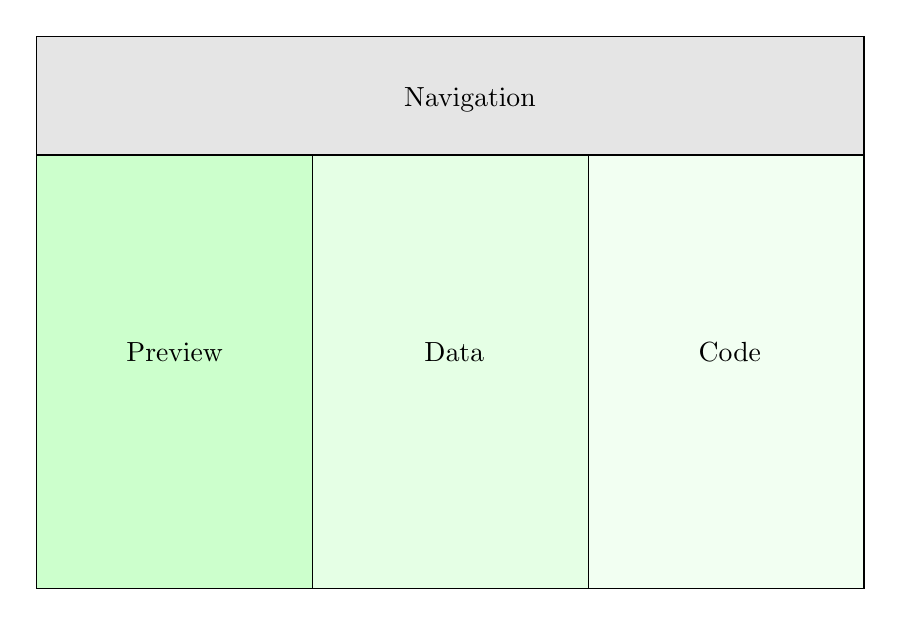
\begin{tikzpicture}
\draw [thick]  (-3,2.5) node (v1) {} rectangle (7.5,-4.5) node (v4) {};
\draw [fill=gray!20!white] (v1) rectangle (7.5,1);
\draw [fill=green!20] (-3,1) rectangle (0.5,-4.5) node (v2) {};
\draw [fill=green!10] (v2) rectangle (4,1) node (v3) {};
\draw [fill=green!5] (v3) rectangle (v4);
\node at (2.5,1.7) {Navigation};
\node at (5.8,-1.5) {Code};
\node at (2.3,-1.5) {Data};
\node at (-1.25,-1.5) {Preview};
\end{tikzpicture}
\end{document}